\documentclass{article}

\usepackage[%
  papersize={8.25cm,7.25cm},
  hmargin=0cm,%
  vmargin=0cm,%
  head=0cm,% might be changed later
  headsep=0pt,%
  foot=0cm% might be changed later
  ]{geometry}

\usepackage[dvipsnames]{xcolor} % for color palettes
\usepackage{etex}       % changes how LaTex allocates registers (needed for pgfplots)
\usepackage{pgfplots}   % for drawing plots
\usepackage{charter}    % sets font as bitstream charter
\usepackage{filecontents}
\usetikzlibrary{patterns,external}
\usepgfplotslibrary{colormaps}

\pgfplotsset{compat=1.9}

\pagestyle{empty}

\newcommand{\MTSA}{{\scshape mtsa}}
\newcommand{\SUP}{{\scshape supremica}}
\newcommand{\MBP}{{\scshape mbp}}
\newcommand{\SLUGS}{{\scshape slugs}}
\newcommand{\MYND}{{\scshape mynd}}
\newcommand{\PRP}{{\scshape prp}}
\newcommand{\RA}{{\scshape dcs-ra}}
\newcommand{\RAnew}{{\scshape dcs2-ra}}
  
\begin{document}

\begin{figure}
\centering

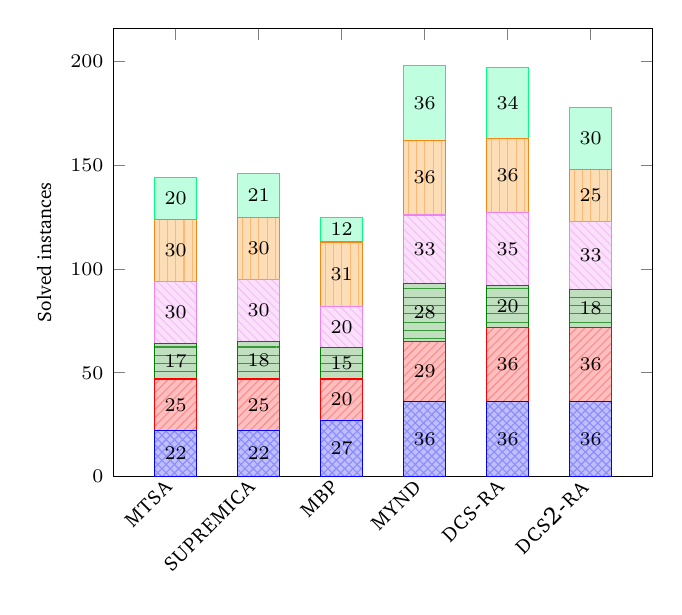
\begin{tikzpicture}
\begin{axis}[
  ybar stacked,
  bar width=15pt,
  nodes near coords,
  enlarge x limits=0.15,
  ymin=0,
  ymax=216,
  font=\scriptsize,
  xticklabel style={font=\small},
  ylabel={Solved instances},
  symbolic x coords={\MTSA,\SUP,\MBP,\MYND,\RA,\RAnew},
  xtick=data,
  x tick label style={rotate=45,anchor=east},
]
\addplot+[ybar,color=blue,fill=blue!25,text=black,postaction={pattern=crosshatch,pattern color=blue!45}]
  plot coordinates {(\MTSA,22) (\SUP,22) (\MBP,27) (\MYND,36) (\RA,36) (\RAnew,36)}; % TL
\addplot+[ybar,color=red,fill=red!25,text=black,postaction={pattern=north east lines,pattern color=red!45}]
  plot coordinates {(\MTSA,25) (\SUP,25) (\MBP,20) (\MYND,29) (\RA,36) (\RAnew,36)}; % DP
\addplot+[ybar,color=Green,fill=Green!25,text=black,postaction={pattern=horizontal lines,pattern color=ForestGreen!90}]
  plot coordinates {(\MTSA,17) (\SUP,18) (\MBP,15) (\MYND,28) (\RA,20) (\RAnew,18)}; % CM
\addplot+[ybar,color=Violet,fill=Violet!25,text=black,postaction={pattern=north west lines,pattern color=Violet!50}]
  plot coordinates {(\MTSA,30) (\SUP,30) (\MBP,20) (\MYND,33) (\RA,35) (\RAnew,33)}; % AT
\addplot+[ybar,color=BurntOrange,fill=BurntOrange!25,text=black,postaction={pattern=vertical lines,pattern color=BurntOrange!55}]
  plot coordinates {(\MTSA,30) (\SUP,30) (\MBP,31) (\MYND,36) (\RA,36) (\RAnew,25)}; % BW
\addplot+[ybar,color=SpringGreen,fill=SpringGreen!25,text=black]
  plot coordinates {(\MTSA,20) (\SUP,21) (\MBP,12) (\MYND,36) (\RA,34) (\RAnew,30)}; % TA
\end{axis}
\end{tikzpicture}
\end{figure}

\end{document}
